The main purpose of this chapter is to provide the reader with all the theoretical information about phosphorylation, kinases, phosphatases and substrates, which is essential in order to be able to understand the scope of this project, its aims and its implementation.
Of course, this section does not provide a detailed description of all properties, functions and behaviour of the aforementioned  molecules and reactions.
If the reader wishes to gain a deeper understanding of the role that these molecules play in a living cell, we refer the reader to \cite{introphosphorylation}.

% Phosphorylation section.
\section{Phosphorylation}
Phosphorylation is a chemical reaction in which a phosphate group ($PO_4$) is added to a biological molecule.
This molecule can be a protein, a lipid or any other kind of organic molecule.
Protein phosphorylation is one of the most common post-translational modifications of proteins and it plays a significant role in a wide variety of cellular processes in eukaryotic and prokaryotic cells, including cellular growth, differentiation and DNA repair \cite{phosphoELM}.
In eukaryotic cells phosphorylation occurs mainly on Serine, Threonine and Tyrosine amino acids, whereas in prokaryotic cells it occurs mainly on Histidine, Arginine and Lysine residues.

\begin{figure}[ht]
\centering
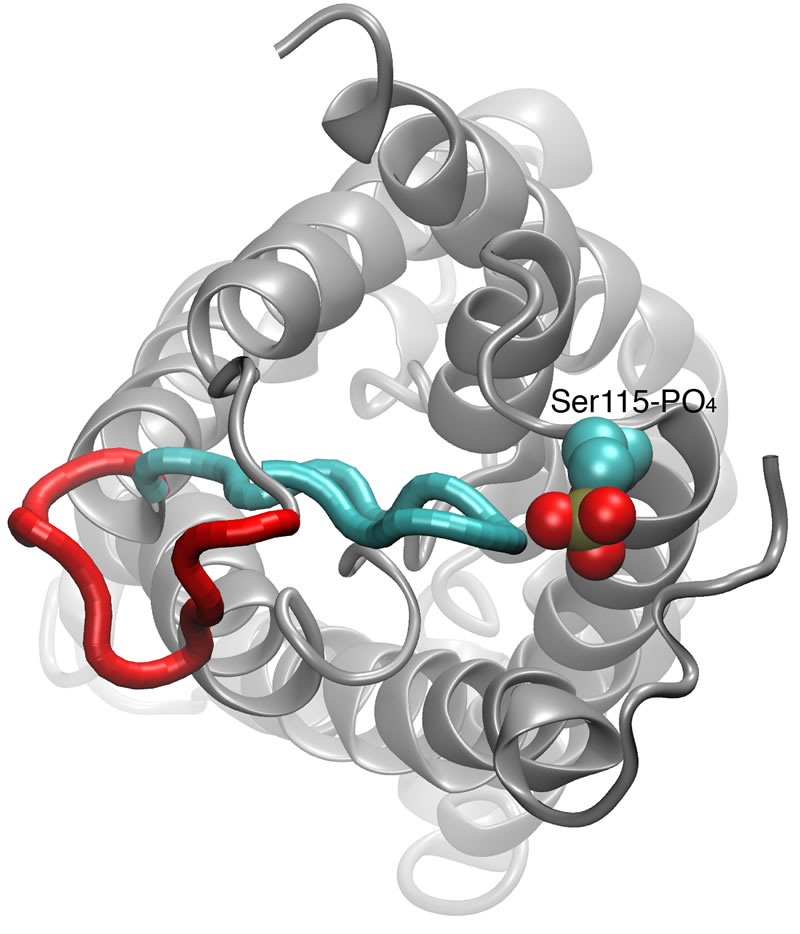
\includegraphics{pictures/phosphorylation.png}
\caption[The effects of phosphorylation]{The effects of phosphorylation to aquaporin SoPIP2. (Courtesy Yi Wang)}
\label{Phosphorylation}
\end{figure}

In eukaryotic cells, phosphorylation tightly regulates the dynamic behaviour and decision processes of the cell.
It can modify protein function by introducing conformational changes or by creating new binding sites for protein-protein interaction domains that recognize phosphorylated motifs and bind to them \cite{networKIN}.
One example of a conformational change to the aquaporin SoPIP2;1 after phosphorylation is illustrated in Figure \ref{Phosphorylation}.
Aquaporins are membrane proteins specialized in transporting water molecules across biological membranes.
They are highly efficient and they are able to transport more than a billion water molecules per second.
Most aquaporins in animals are always in an open state, allowing water to easily pass through them.
On the contrary, plant aquaporins constantly change states according to signals, such as phosphorylation and pH, enabling plant cells to respond to drastic changes in their environment.
Figure \ref{Phosphorylation} shows how aquaporin SoPIP2;1, commonly found in spinach, can switch from the closed to the open state after phosphorylation.
As the Serine residue (Ser115) undergoes phosphorylation, the loop moves away from the entrance of the water channel and water molecules are able to move freely through it \cite{aquaporin}.
The unphosphorylated state is shown in cyan, whereas the phosphorylated state is shown in red.

Phosphorylation events take place only in certain sites, namely phosphorylation sites, which mainly consist of the protein residue that undergoes phosphorylation and its neighbouring amino acids.
These sites are commonly located in parts of a protein where the accessibility and structural flexibility are rather high, for example loops and hinges.
This fact makes it easier for other biological molecules, such as kinases and phosphatases, to access them and catalyze the phosphorylation reaction \cite{PHOSIDA}.
Moreover, since the rate of mutation in these parts of a protein is comparatively high, the sequence regions around the residue subject to phosphorylation are evolving faster than the rest of the protein.
Therefore it is difficult to correctly align phosphorylation sites found in homologous proteins and positively identify them.

A lot of effort has been invested by the scientific community to find phosphosites in proteins and annotate them, because this information offers insight to the various signaling pathways that each protein takes part in.
Traditional methods for locating phosphorylation sites include Edman degradation chemistry on phosphopeptides and mutational analysis.
These methods require large amounts of purified protein and they are relatively time consuming.
The aforementioned disadvantages have led scientists to use modern Mass Spectrometry based methods to locate novel phosphosites in proteins and analyze protein post-translational modifications.
These techniques offer higher sensitivity and speed and they are able to generate high quality data \cite{phosphoELM}.

In previous years, thousands of phosphorylation sites have been identified using the methods and techniques described before.
As a consequence, a lot of bioinformatics databases have been created in order to store all these data.
Nevertheless, the information on which kinases act on these sites and the pathways that each protein is involved in is still missing.
KiPhoDB aims to fill this gap and provide scientists with a valuable resource of information that can be easily accessed by the scientific community.

It has been estimated that almost one third of all proteins undergo phosphorylation at some point in their lifetime \cite{kinomics}.
Each protein may contain one or more phosphorylation sites, which are regulated by one or more other proteins.
The processes of phosphorylation and dephosphorylation of a protein are two ways to change its state from `activated' to `deactivated' and vice versa.
These processes play a key role in signal transduction and in various other metabolic and cellular pathways.
Therefore, the scientific community has adopted different approaches to elucidate and understand them.
One such global approach is the field of 'Phosphoproteomics', which is dedicated to identifying and quantifying dynamic changes in phosphorylated proteins over time using mass spectrometry.
These techniques are becoming increasingly important for the systematic analysis of complex phosphorylation networks.

The deregulation of protein phosphorylation and dephosphorylation in a particular pathway leads to various anomalies in cell function, which are responsible for the emergence of diseases.
One such example is the p53 tumor suppressor protein \cite{p53tumorsuppressor}, which is activated by phosphorylation and suppresses tumors by causing cell cycle arrest (Apopotosis).
Thus phosphorylated p53 is the central defence of a cell against cancer.
This highlights the importance of phosphorylation from a medical point of view (e.g. potential drug targets), apart from its relevant importance in molecular and cell biology.

In the following sections we will examine two different kind of molecules: Kinases and Phosphatases.
Protein kinases are responsible for the phosphorylation of substrates, whereas protein phosphatases are involved in the dephosphorylation of substrates.

% Kinase section.
\section{Kinase}
Kinase is a type of enzyme that transfers phosphate groups from high energy donor molecules, such as ATP, to specific target molecules, namely substrates.
They are also known as phosphotransferases and they can act on more than one phosphorylation sites on the surface of a given substrate.
Kinases play central roles in various important cellular and metabolic networks (e.g. signal transduction, cellular growth and apoptosis), where they are often associated with the activation or deactivation of other proteins.
Apart from proteins, kinases can also act in other small molecules, such as lipids, nucleotides, carbohydrates and others.

\begin{figure}[hp]
\centering
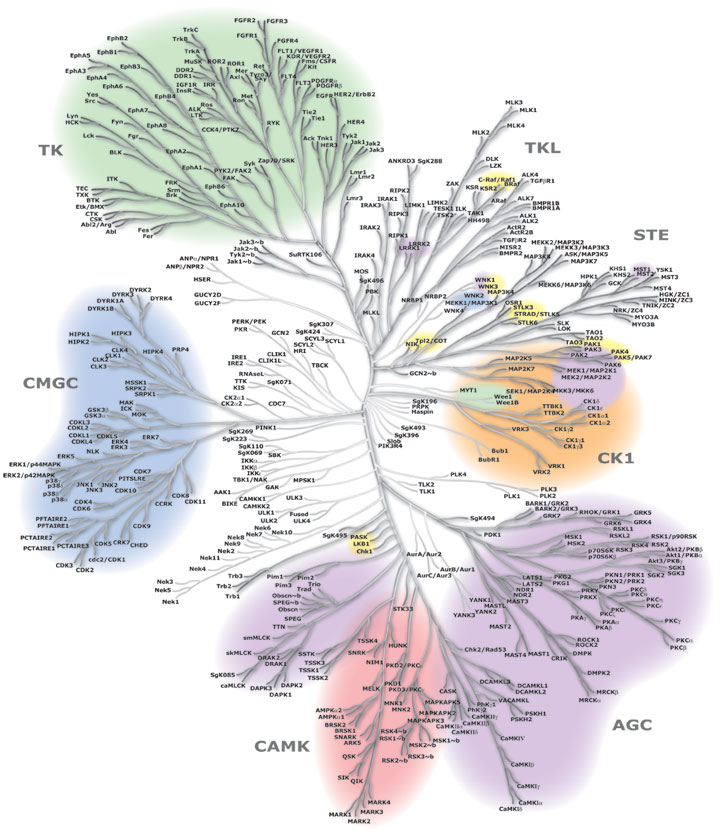
\includegraphics[scale=0.6]{pictures/kinome.png}
\caption{The human kinome.}
\label{Kinome}
\end{figure}

\begin{figure}[ht]
\centering
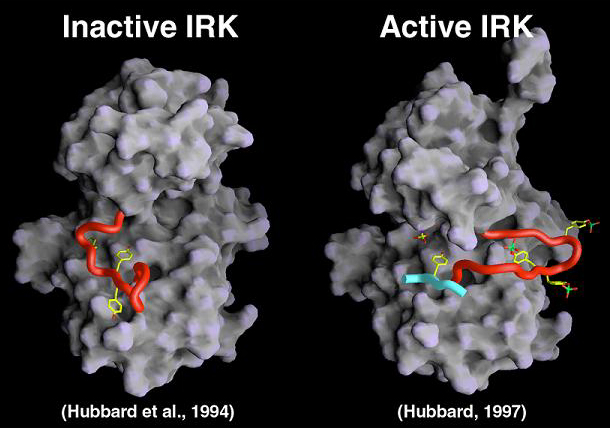
\includegraphics[scale=0.5]{pictures/phosphorylated_kinase.png}
\caption[Insulin Receptor Tyrosine Kinase.]{Activated and deactivated states of Insulin Receptor Tyrosine Kinase. (Courtesy of Stevan R.Hubbard)}
\label{PhosphorylatedKinase}
\end{figure}

It is quite common for kinases to get phosphorylated by other kinase proteins or even catalyze their own phosphorylation (autophosphorylation).
A lot of kinases are activated by phosphorylation on their `activation loop', which is located at the center of most of them.
Figure \ref{PhosphorylatedKinase} illustrates this point.
In this figure, both activated and deactivated states of the protein `insulin receptor tyrosine kinase' are presented.

At the time of writing, up to 518 distinct kinases have been identified in humans \cite{kinome}.
However the scientific community does not know which of these kinases are responsible for which phosphorylation events.
It has been reported \cite{networKIN} that the substrates and exact phosphorylation reactions of only approximately one third (35\%) of the total number of human kinases are known.
Of course this fraction is lower for other species that have not been so thoroughly researched and it is constantly decreasing as more and more phosphorylation sites are identified.
Consequently there is a widening gap in our understanding of phosphorylation networks and signaling pathways, which is very difficult to close.
One of KiPhoDB's aims is to aid scientists in their efforts to investigate phosphorylation networks and help them close this knowledge gap.

\begin{table}[h]
\begin{center}
\vspace{1cm}
\begin{tabular}{ | c | c | c | c |}
\hline
\multicolumn{4}{|c|}{\textbf{Kinase Groups}} \\
\hline
\hline
AGC & CAMK & CK1 & CMGC \\
\hline
Other & STE & Tyrosine Kinase & RGC \\
\hline
Tyrosine Kinase-like & Atypical-PDHK & Atypical-Alpha & Atypical-RIO \\
\hline
Atypical-A6 & Atypical-Other & Atypical-ABC1 & Atypical-BRD \\
\hline
Atypical-PIKK & & & \\
\hline
\end{tabular}
\end{center}
\caption[Kinase group classification.]{Kinase group classification \cite{kinome}.}
\label{table:Kinases}
\end{table}

Kinases are among the largest gene families in eukaryotes and according to \cite{kinome} they can be classified in the kinase groups shown in Table \ref{table:Kinases}.
As shown in this table, there are seventeen major groups of kinases, which in turn have their own subcategories (families).
This classification schema proves that kinases are enormously diverse.
Figure \ref{Kinome} further illustrates this point by presenting the human kinome in the form of a tree.
In this figure, all previously mentioned groups are shown painted with different colour, along with their subgroups.
Mutations to these molecules may cause disease in human and other species and therefore kinases are attractive targets for drug design.

\begin{figure}[h]
\centering
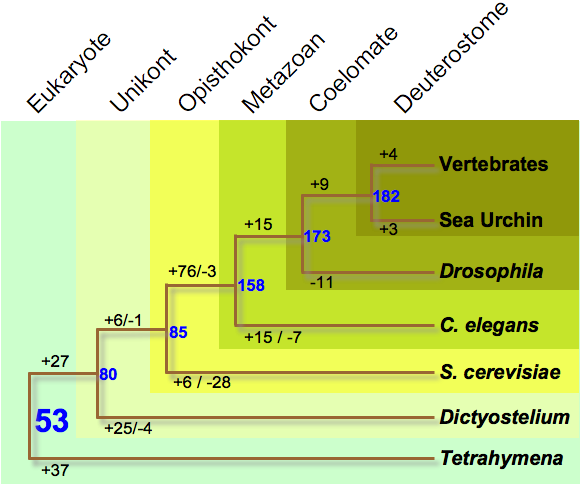
\includegraphics[scale=0.5]{pictures/subfamily_tree.png}
\caption[The evolution of kinases in different species.]{The evolution of kinases in different species (Courtesy of Manning et al).}
\label{evolution_kinases}
\end{figure}

The majority of protein kinases belong to a single superfamily and they share the same catalytic domain, namely ePK (eukaryotic Protein Kinase).
Nevertheless, there are thirteen additional atypical protein kinase families (aPK - atypical Protein Kinases) which exhibit biochemical kinase activity, although they do not contain the ePK domain.
However it has been reported \cite{kinome} that these kinases have some common structural characteristics with the ePK domain.
Whole kinome comparisons have enabled scientists to compare kinases across highly diverse species and have helped in the analysis of birth, spread, expansion and even death of kinases.
Results from such analyses have shown that there were around 53 distinct kinase functions in the early common ancestor of all eukaryotes \cite{kinase_evolution}.
In the present day we find that there has been a lot of gain and loss in the kinase types across all species.
This is clearly illustrated in Figure \ref{evolution_kinases}, which presents the evolution of kinases in a variety of species.
As it is clearly shown in this figure, the most dramatic change is the emergence of metazoans with 76 classes of kinases, including among others the tyrosine kinase group.
On the contrary, there have been only 28 classes in yeast which have also emerged from the ancestral kinase groups.
The evolutionary analysis of all kinases in form of trees curated at various databases can help understand the evolution of various metabolic pathways in many organisms.

% Phosphatase section.
\section{Phosphatase}
A phosphatase is an enzyme whose action is directly opposite to that of a kinase.
Its main function is to remove a phosphate group from the given substrate, a process also known as dephosphorylation, which is the complement of the phophorylation done by kinases.
Phoshatases, together with kinases, are involved in important dynamic control and communication mechanisms inside a living cell.
These mechanisms include metabolism, cell signaling, cell growth, muscle contraction, homeostasis and many more.
It has also been proven that phosphatase malfunction may cause a wide variety of diseases in humans, such as diabetes, many types of cancer and obesity \cite{phosphabase}.
Therefore, as stated in previous sections, both protein kinases and protein phosphatases are important targets for molecular biology, pharmaceutical and medical research.
For more information on the diverse roles that phosphatases play in living cells, we refer the reader to \cite{nuclear_phosphatases}, where all presently known phosphatase functions are thoroughly reviewed.

For a long time, phosphatases were viewed by the scientific community as passive housekeeping enzymes.
Yet in the last few years this view has started to change and now kinases and phosphatases are thought to be partners, both regulating the responses to certain signals.
Recent studies indicate that kinases play a major role in controlling the timing and the amplitute of a signalling response, whereas phosphatases control mostly the rate and the duration of the response \cite{tyrosine_phosphatases}.
This behaviour of kinases and phosphatases is presented in Figure \ref{phosphorylation_dephosphorylation}.

\begin{figure}[ht]
\centering
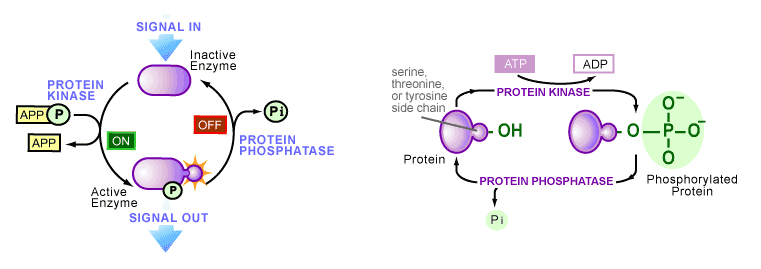
\includegraphics[scale=0.6]{pictures/phosphorylation_dephosphorylation.png}
\caption[The role of kinases and phosphatases in signalling pathways.]{The role of kinases and phosphatases in signalling pathways (Courtesy of David Secko).}
\label{phosphorylation_dephosphorylation}
\end{figure}

There are three main groups of protein phosphatases.
The first group is called protein Ser/Thr phosphatase and it consists of phosphatases that dephosphorylate either Serine or Threonine amino acids.
This group is further divided into the following families: the large phosphoprotein phosphatase (PPP) family and the $Mg^{2+}$ or $Mn^{2+}$ dependent protein phosphatase family (PP2C).
The second group is called protein Tyr phosphatases and it contains only phosphatases that dephosphorylate Tyrosine residues.
Finally, the third group consists of Asp-based protein phosphatases \cite{nuclear_phosphatases}.

It was stated in the previous section that human DNA encodes 518 protein kinases, 428 of which are known or predicted to phosphorylate Serine and Threonine residues, whereas ony 90 of them phosphorylate Tyrosine.
On the contrary there are only 147 protein phosphatases encoded in the human genome, 107 of which desphosphorylate Tyrosine amino acids and only 40 of them dephosphorylate Serine and Threonine residues.
This discovery is very strange because, as we will see in more detail in the next section, more than 98\% of the phosphorylation events take place on Serine and Threonine side chains.
Therefore, the vast majority of phosphorylation events are dephosphorylated by only 40 of the 147 known phosphatases \cite{nuclear_phosphatases}. 

% Substrate
\section{Substrate}
Substrates are acted upon by kinases and phosphatases and they contain phosphorylation sites which bind a phosphate group to a particular amino acid.
As it was clearly illustrated in the previous sections, kinases and phosphatases can themselves be substrates.
For example, some kinase cascades have been discovered where each given kinase is itself a substrate to the previous kinase and at the same time phosphorylates the next kinase in the cascade.

\begin{figure}[ht]
\centering
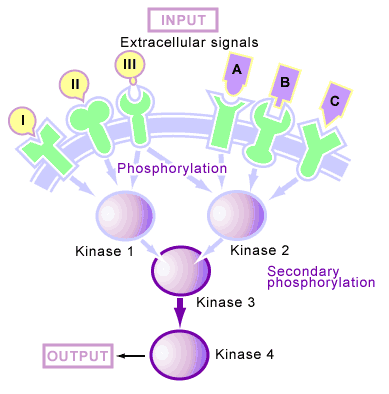
\includegraphics[scale=0.6]{pictures/phosphorylation_cascade.png}
\caption[A phosphorylation cascade.]{A phosphorylation cascade (Courtesy of David Secko).}
\label{phosphorylation_cascade}
\end{figure}

One such cascade is presented in Figure \ref{phosphorylation_cascade}.
In this figure it is clearly illustrated how extracellular signals are received by specific transmembrane sensing proteins and how these proteins cause the phosphorylation of kinases.
Subsequently these kinases phosphorylate other protein kinases leading to the creation of a phosphorylation cascade, which at the end transfers the signal to the appropriate receiver protein.
The phosphorylation cascade continues to function until the corresponding protein phosphatases are activated and manage to shut it down.

It is important to note at this point that phosphorylation events happen to only three out of a total of twenty amino acids.
These amino acids are Serine (Ser), Threonine (Thr) and Tyrosine (Tyr) and their frequencies for the human phosphoproteome are presented in Figure \ref{phosphorylation_site_graph}.
The percentage for Serine is 86.4\%, for Threonine is 11.8\% and for Tyrosine is 1.8\% \cite{nuclear_phosphatases}.
Of course these percentages vary in different species.

\begin{figure}[ht]
\centering
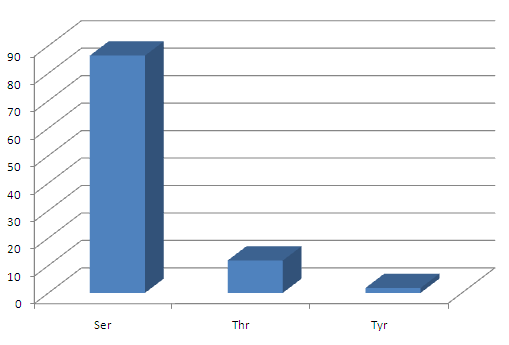
\includegraphics[scale=0.5]{pictures/phosphorylation_site_graph.png}
\caption{The frequencies of different kinds of phosphorylation sites.}
\label{phosphorylation_site_graph}
\end{figure}

It is widely known that phosphate groups are negatively charged and each one of them carries two negative charges.
Therefore their addition to a protein through the process of phosphorylation may change the protein's structure and its overall behaviour.
Nevertheless, once the protein gets dephosphorylated and the phosphate group is removed, the protein switches back to its original conformation.
In most cases, these conformational changes result to changes in the protein's function and therefore phosphorylation and dephosphorylation can act as a molecular switch, turning a specific activity on and off.
This mechanism of changing proteins' behaviour has many advantages: it is very rapid, taking only a few seconds, and it does not involve the destruction or creation of new proteins.
Moreover, it is easily reversible and thus this fact makes the whole mechanism more flexible. 

The advantages of the phosphorylation/dephosphorylation mechanism explain its extensive use as a control mechanism for various processes within a living cell.
For example it has been proven that approximately 3\% of the total number of proteins in yeast are kinases or phosphatases.
Some of these enzymes are able to act on a wide variety of target proteins, while others are extremely specific and act only on a few substrates.
These substrates include other enzymes, ion channels, cell receptors, structural proteins and many more.
Furthermore, the research in phosphorylation, kinases, phosphatases and substrates has been very active and intense the last few years, especially since 1992 when Fischer and Krebs, two pioneers on this field, received the Nobel Prize in medicine for their contribution \cite{phosphorylation_origins}. 


